\documentclass{standalone}
\usepackage{tikz}
\usetikzlibrary{patterns, positioning}
\usepackage[sfdefault]{ClearSans} %% option 'sfdefault' activates Clear Sans as the default text font
\usepackage[T1]{fontenc}

\begin{document}
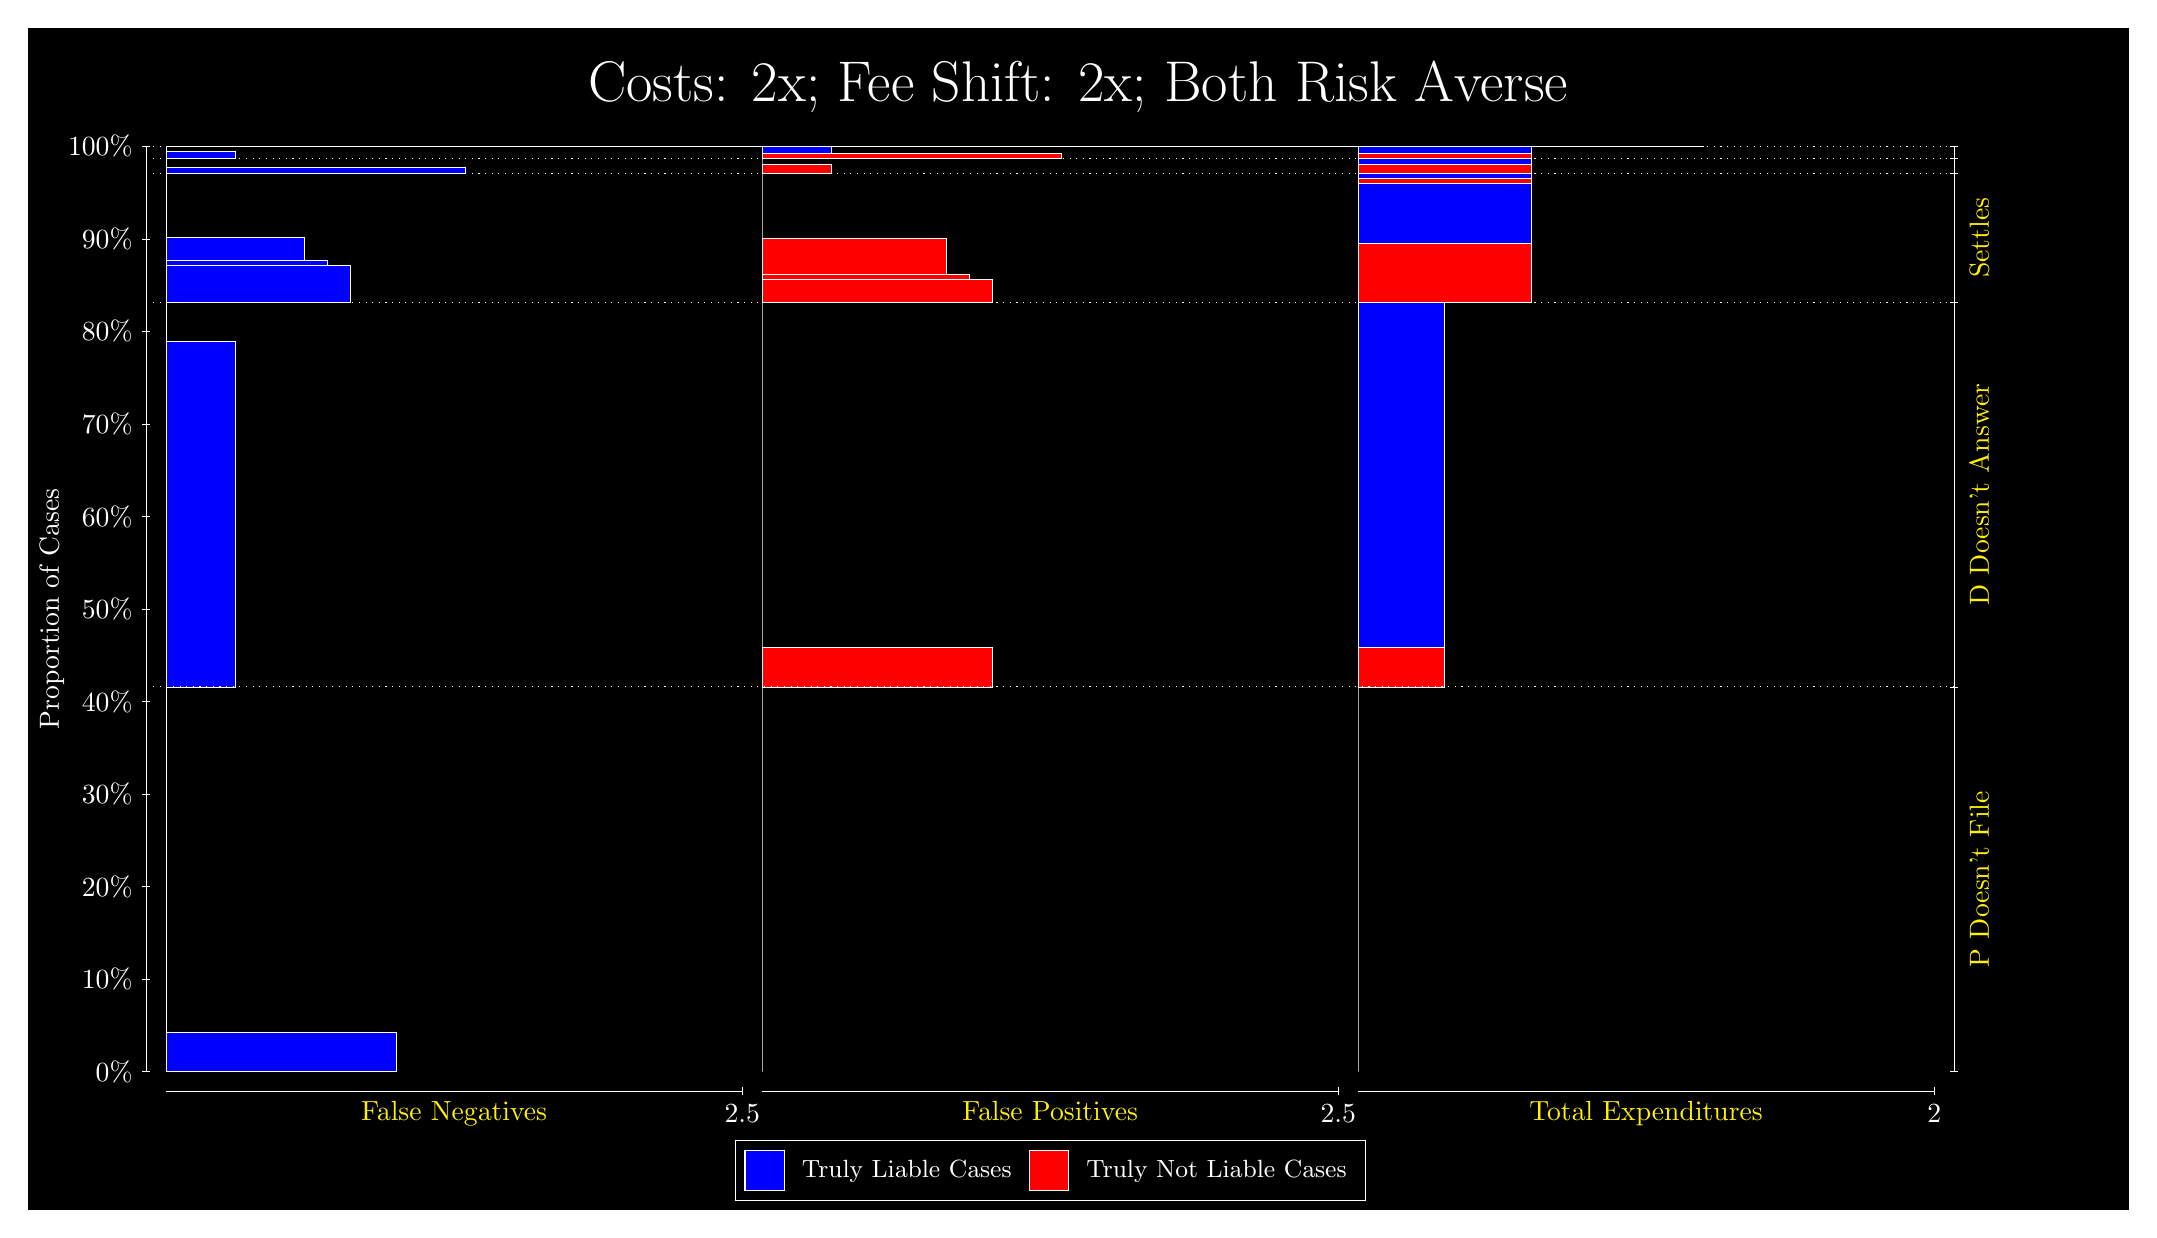
\begin{tikzpicture}
\draw[fill=black] (0,0) rectangle (26.667,15);
\draw[text=white] (0,13.5) rectangle (26.667,15) node[midway] {\huge Costs: 2x; Fee Shift: 2x; Both Risk Averse};
\draw[white, very thin] (1.5,1.75) -- (1.5,13.5);
\node[rotate=90, text=white, anchor=center] at (0.3, 7.625) {Proportion of Cases};
\draw[white, very thin] (1.45,1.75) -- (1.55,1.75);
\node[text=white, anchor=east] at (1.45, 1.75) {0\%};
\draw[white, very thin] (1.45,2.925) -- (1.55,2.925);
\node[text=white, anchor=east] at (1.45, 2.925) {10\%};
\draw[white, very thin] (1.45,4.1) -- (1.55,4.1);
\node[text=white, anchor=east] at (1.45, 4.1) {20\%};
\draw[white, very thin] (1.45,5.275) -- (1.55,5.275);
\node[text=white, anchor=east] at (1.45, 5.275) {30\%};
\draw[white, very thin] (1.45,6.45) -- (1.55,6.45);
\node[text=white, anchor=east] at (1.45, 6.45) {40\%};
\draw[white, very thin] (1.45,7.625) -- (1.55,7.625);
\node[text=white, anchor=east] at (1.45, 7.625) {50\%};
\draw[white, very thin] (1.45,8.8) -- (1.55,8.8);
\node[text=white, anchor=east] at (1.45, 8.8) {60\%};
\draw[white, very thin] (1.45,9.975) -- (1.55,9.975);
\node[text=white, anchor=east] at (1.45, 9.975) {70\%};
\draw[white, very thin] (1.45,11.15) -- (1.55,11.15);
\node[text=white, anchor=east] at (1.45, 11.15) {80\%};
\draw[white, very thin] (1.45,12.325) -- (1.55,12.325);
\node[text=white, anchor=east] at (1.45, 12.325) {90\%};
\draw[white, very thin] (1.45,13.5) -- (1.55,13.5);
\node[text=white, anchor=east] at (1.45, 13.5) {100\%};

\draw[white, very thin] (24.457,1.75) -- (24.457,13.5);
\draw[white, very thin] (24.407,1.75) -- (24.507,1.75);
\node[anchor=west] at (24.407, 1.75) {};
\draw[white, very thin] (24.407,6.6358) -- (24.507,6.6358);
\node[anchor=west] at (24.407, 6.6358) {};
\draw[white, very thin] (24.407,11.521) -- (24.507,11.521);
\node[anchor=west] at (24.407, 11.521) {};
\draw[white, very thin] (24.407,13.16) -- (24.507,13.16);
\node[anchor=west] at (24.407, 13.16) {};
\draw[white, very thin] (24.407,13.35) -- (24.507,13.35);
\node[anchor=west] at (24.407, 13.35) {};
\draw[white, very thin] (24.407,13.499) -- (24.507,13.499);
\node[anchor=west] at (24.407, 13.499) {};
\draw[white, very thin] (24.407,13.499) -- (24.507,13.499);
\node[anchor=west] at (24.407, 13.499) {};
\draw[white, very thin] (24.407,13.5) -- (24.507,13.5);
\node[anchor=west] at (24.407, 13.5) {};

\draw[white, very thin, fill=blue] (1.75,1.75) rectangle (4.6775,2.2488);
\draw[white, very thin, fill=red] (1.75,2.2488) rectangle (1.75,6.6358);
\draw[white, very thin, fill=blue] (1.75,6.6358) rectangle (2.6283,11.022);
\draw[white, very thin, fill=red] (1.75,11.022) rectangle (1.75,11.521);
\draw[white, very thin, fill=blue] (1.75,11.521) rectangle (4.092,11.988);
\draw[white, very thin, fill=blue] (1.75,11.988) rectangle (3.7993,12.057);
\draw[white, very thin, fill=blue] (1.75,12.057) rectangle (3.5065,12.344);
\draw[white, very thin, fill=red] (1.75,12.344) rectangle (1.75,13.16);
\draw[white, very thin, fill=blue] (1.75,13.16) rectangle (5.5558,13.238);
\draw[white, very thin, fill=red] (1.75,13.238) rectangle (1.75,13.35);
\draw[white, very thin, fill=blue] (1.75,13.35) rectangle (2.6283,13.437);
\draw[white, very thin, fill=red] (1.75,13.437) rectangle (1.75,13.499);
\draw[white, very thin, fill=blue] (1.75,13.499) rectangle (9.9471,13.499);
\draw[white, very thin, fill=red] (1.75,13.499) rectangle (1.75,13.499);
\draw[white, very thin, fill=red] (1.75,13.499) rectangle (1.75,13.5);
\draw[white, very thin, fill=blue] (1.75,13.5) rectangle (1.75,13.5);
\draw[white, very thin, fill=red] (9.3189,1.75) rectangle (9.3189,6.137);
\draw[white, very thin, fill=blue] (9.3189,6.137) rectangle (9.3189,6.6358);
\draw[white, very thin, fill=red] (9.3189,6.6358) rectangle (12.246,7.134);
\draw[white, very thin, fill=blue] (9.3189,7.134) rectangle (9.3189,11.521);
\draw[white, very thin, fill=red] (9.3189,11.521) rectangle (12.246,11.807);
\draw[white, very thin, fill=red] (9.3189,11.807) rectangle (11.954,11.871);
\draw[white, very thin, fill=red] (9.3189,11.871) rectangle (11.661,12.337);
\draw[white, very thin, fill=blue] (9.3189,12.337) rectangle (9.3189,13.16);
\draw[white, very thin, fill=red] (9.3189,13.16) rectangle (10.197,13.271);
\draw[white, very thin, fill=blue] (9.3189,13.271) rectangle (9.3189,13.35);
\draw[white, very thin, fill=red] (9.3189,13.35) rectangle (13.125,13.412);
\draw[white, very thin, fill=blue] (9.3189,13.412) rectangle (10.197,13.499);
\draw[white, very thin, fill=red] (9.3189,13.499) rectangle (9.3189,13.499);
\draw[white, very thin, fill=blue] (9.3189,13.499) rectangle (9.3189,13.499);
\draw[white, very thin, fill=red] (9.3189,13.499) rectangle (17.516,13.5);
\draw[white, very thin, fill=blue] (9.3189,13.5) rectangle (14.588,13.5);
\draw[white, very thin, fill=red] (16.888,1.75) rectangle (16.888,6.137);
\draw[white, very thin, fill=blue] (16.888,6.137) rectangle (16.888,6.6358);
\draw[white, very thin, fill=red] (16.888,6.6358) rectangle (17.986,7.134);
\draw[white, very thin, fill=blue] (16.888,7.134) rectangle (17.986,11.521);
\draw[white, very thin, fill=red] (16.888,11.521) rectangle (19.083,12.273);
\draw[white, very thin, fill=blue] (16.888,12.273) rectangle (19.083,13.027);
\draw[white, very thin, fill=red] (16.888,13.027) rectangle (19.083,13.091);
\draw[white, very thin, fill=blue] (16.888,13.091) rectangle (19.083,13.16);
\draw[white, very thin, fill=red] (16.888,13.16) rectangle (19.083,13.271);
\draw[white, very thin, fill=blue] (16.888,13.271) rectangle (19.083,13.35);
\draw[white, very thin, fill=red] (16.888,13.35) rectangle (19.083,13.412);
\draw[white, very thin, fill=blue] (16.888,13.412) rectangle (19.083,13.499);
\draw[white, very thin, fill=red] (16.888,13.499) rectangle (21.279,13.499);
\draw[white, very thin, fill=blue] (16.888,13.499) rectangle (21.279,13.499);
\draw[white, very thin, fill=red] (16.888,13.499) rectangle (21.279,13.5);
\draw[white, very thin, fill=blue] (16.888,13.5) rectangle (21.279,13.5);
\draw[white, dotted] (1.5,6.6358) -- (24.457,6.6358);
\draw[white, dotted] (1.5,11.521) -- (24.457,11.521);
\draw[white, dotted] (1.5,13.16) -- (24.457,13.16);
\draw[white, dotted] (1.5,13.35) -- (24.457,13.35);
\draw[white, dotted] (1.5,13.499) -- (24.457,13.499);
\draw[white, dotted] (1.5,13.499) -- (24.457,13.499);
\draw[white, very thin] (1.75,1.5) -- (9.0689,1.5);
\node[text=yellow, anchor=north] at (5.4094, 1.5) {False Negatives};
\draw[white, very thin] (9.0689,1.45) -- (9.0689,1.55);
\node[text=white, anchor=north] at (9.0689, 1.45) {2.5};

\draw[white, very thin] (9.3189,1.5) -- (16.638,1.5);
\node[text=yellow, anchor=north] at (12.978, 1.5) {False Positives};
\draw[white, very thin] (16.638,1.45) -- (16.638,1.55);
\node[text=white, anchor=north] at (16.638, 1.45) {2.5};

\draw[white, very thin] (16.888,1.5) -- (24.207,1.5);
\node[text=yellow, anchor=north] at (20.547, 1.5) {Total Expenditures};
\draw[white, very thin] (24.207,1.45) -- (24.207,1.55);
\node[text=white, anchor=north] at (24.207, 1.45) {2};

\node[text=yellow, centered, rotate=90] at (24.777, 4.1929) {P Doesn't File};
\node[text=yellow, centered, rotate=90] at (24.777, 9.0782) {D Doesn't Answer};
\node[text=yellow, centered, rotate=90] at (24.777, 12.34) {Settles};





\draw (12.978300999999998,1.5) node[draw=none] (baseCoordinate) {};
\begin{scope}[align=center]
        \matrix[scale=0.5, draw=white, below=0.5cm of baseCoordinate, nodes={draw}, column sep=0.1cm]{
            \node[rectangle, draw, minimum width=0.5cm, minimum height=0.5cm, fill=blue] {}; &
            \node[draw=none, font=\small, text=white] (B) {Truly Liable Cases}; &
            \node[rectangle, draw, minimum width=0.5cm, minimum height=0.5cm, fill=red] {}; &
            \node[draw=none, font=\small, text=white] (B) {Truly Not Liable Cases}; \\
            };
\end{scope}

\end{tikzpicture}
\end{document}